%
% HICSS-60 제출 논문 — 한국어 번역본 (내부 검토용)
% 영문 원본: hicss_paper.tex
%
\documentclass[10pt]{article}
%
% hicss-packages.tex
% HICSS-60 compatible package and layout settings
% Based on HICSS official formatting guidelines (10pt, Times, two-column, 1-inch margins)
%

% --- Page geometry ---
\usepackage[letterpaper,
            top=1in, bottom=1in,
            left=1in, right=1in]{geometry}

% --- Two-column layout ---
\usepackage{multicol}
\twocolumn
\setlength{\columnsep}{0.33in}

% --- Fonts ---
\usepackage{times}
\usepackage[T1]{fontenc}
\usepackage[utf8]{inputenc}

% --- Math ---
\usepackage{amsmath,amssymb}

% --- Graphics ---
\usepackage{graphicx}
\usepackage[table]{xcolor}   % required for \cellcolor in tables

% --- Tables ---
\usepackage{booktabs}
\usepackage{multirow}
\usepackage{array}
\usepackage{tabularx}

% --- Prevent text overflowing column ---
\emergencystretch=2em

% --- Bibliography (biblatex + bibtex) ---
\usepackage[backend=bibtex,
            style=authoryear,
            sorting=nyt,
            maxbibnames=6,
            minbibnames=3,
            uniquename=false,
            uniquelist=false]{biblatex}

% --- Hyperlinks (load last) ---
\usepackage[colorlinks=true,
            linkcolor=black,
            citecolor=black,
            urlcolor=black]{hyperref}

% --- Section title formatting ---
\usepackage{titlesec}
\titleformat{\section}{\normalfont\large\bfseries}{\thesection.}{0.5em}{}
\titleformat{\subsection}{\normalfont\normalsize\bfseries}{\thesubsection}{0.5em}{}
\titleformat{\subsubsection}{\normalfont\normalsize\itshape}{\thesubsubsection}{0.5em}{}

% --- Caption formatting ---
\usepackage{caption}
\captionsetup{font=small, labelfont=bf}

% --- Spacing ---
\usepackage{setspace}
\setlength{\parskip}{0pt}
\setlength{\parindent}{1em}

% --- Figure/table placement ---
\usepackage{float}

% --- Checkmark / cross symbols ---
\usepackage{pifont}
\newcommand{\cmark}{\ding{51}}   % heavy checkmark
\newcommand{\xmark}{\ding{55}}   % heavy x

% --- Misc ---
% \usepackage{microtype}  % disabled: causes compile timeout on Overleaf free plan
\usepackage{enumitem}
\setlist[itemize]{topsep=2pt, itemsep=1pt}

\usepackage{kotex}   % Korean support (requires XeLaTeX or LuaLaTeX on Overleaf)
\newcommand{\sansserifformat}[1]{\fontfamily{cmss}{ #1}}%

\addbibresource{references.bib}

\title{비결정적 디지털 트윈에서의 신뢰 가능한 스케줄링을 위한\\
LLM 거버넌스 기반 계층적 DRL}

\date{}

\begin{document}
\maketitle

% ============================ 초록 ============================
\begin{abstract}
\textit{%
심층강화학습(DRL)은 제조 스케줄링 분야에 점점 더 많이 적용되고 있으나,
학습된 정책의 신뢰성 문제가 존재한다. 고충실도 디지털 트윈의 내재적 비결정성으로
인해, 동일하게 설정된 학습 실행이 어떤 경우에는 우수한 정책으로 수렴하고
어떤 경우에는 치명적으로 실패하기도 한다.
본 연구는 반도체 제조 디지털 트윈에서의 긴급 로트 스케줄링을 분석하여,
긴급 로트가 스케줄링 충돌을 야기할 만큼 충분히 빈번한 경우
DRL이 독립 실행의 60\%에서 치명적으로 실패함을 보인다.
본 논문은 로컬 호스팅 대형언어모델(LLM)이 에피소드 단위 거버넌스 계층으로서
DRL 에이전트를 제약하는 안전 룰을 생성하는 3계층 계층적 강화학습(HRL) 프레임워크를
제안한다.
5개의 독립 시드에 걸쳐, Pure DRL은 60\%의 실행에서 실패한 반면
LLM 거버넌스 에이전트는 0\% 실패율을 달성하여, 생산 목표 달성률의 손실 없이
사이클 타임 분산을 73\% 감소시켰다.
LLM 거버넌스를 내결함성 메커니즘으로 정의하여, 사회기술적 제조 시스템에서
학습 컴포넌트의 신뢰성을 향상시킴을 논한다.
}
\end{abstract}

\subsubsection*{키워드:}
신뢰성 AI; 심층강화학습; 대형언어모델; 디지털 트윈; 제조 스케줄링

% ============================ 1. 서론 ============================
\section{서론}

반도체 제조 라인은 확률적이고 비정상적인(non-stationary) 스케줄링
환경이다. 단 하나의 디스패칭 결정이 공정 내 재공품(WIP) 분포를 재편하고,
수십 분에서 수 시간 후의 사이클 타임에 영향을 미칠 수 있다. 따라서 시점
$t$에서 스케줄러의 행동은 고정 휴리스틱으로는 귀속하기도, 최적화하기도
어려운 장기적 결과를 수반한다\cite{moyne2017,hu2019}. 이러한 복잡성에
대처하기 위해 최근 연구들은 라인의 고충실도 이산 이벤트 시뮬레이션인
\emph{디지털 트윈(Digital twin)}과 심층강화학습(DRL)을 결합하여 시뮬레이션
환경에서 직접 디스패칭 정책을 학습하고 있다\cite{waschneck2018,lee2025}.
Figure~\ref{fig:drl_framework}는 이러한 기본 결합 구조를 보여준다: 제조
디지털 트윈이 공장 현장 상태를 제공하고 디스패칭 행동을 수신하는 동안,
Rainbow DQN 에이전트는 Q-네트워크와 타겟 네트워크 쌍을 통해 경험 재플레이로
학습한다.

\begin{figure}[h]
  \centering
  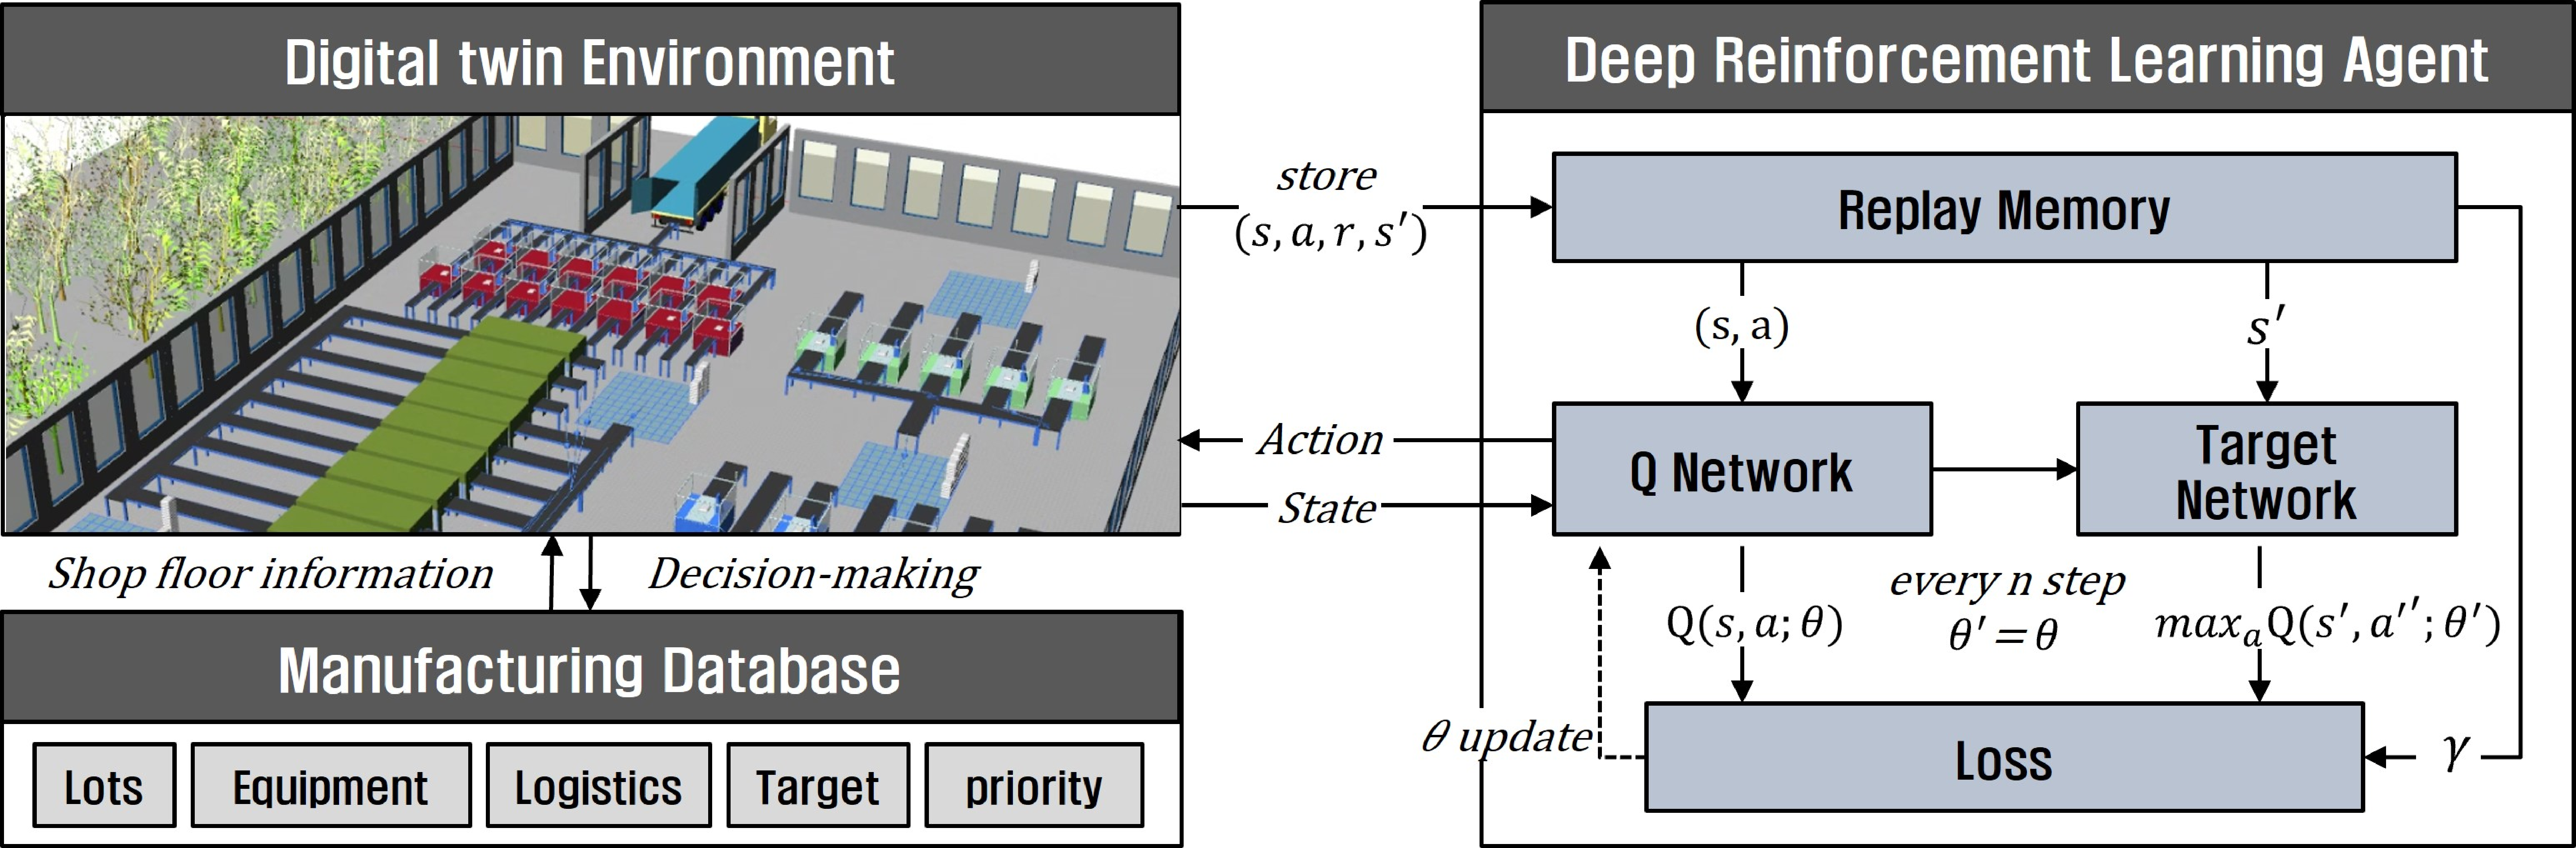
\includegraphics[width=0.98\linewidth]{DRL_Framework}
  \caption{기본 DRL 스케줄링 프레임워크. 디지털 트윈이 학습 환경으로 작동하며,
    에이전트는 공장 현장 상태 $s$를 관찰하고 디스패칭 행동 $a$를 선택한 뒤,
    벨만 손실 $\mathcal{L}(\theta)=\bigl(Q(s,a;\theta)
    -[r+\gamma\max_{a'}Q(s',a'';\theta')]\bigr)^{2}$를 통해
    Q-네트워크 가중치 $\theta$를 갱신하며,
    타겟 네트워크 $\theta'$는 매 $n$ 스텝마다 동기화된다.}
  \label{fig:drl_framework}
\end{figure}

고무적인 평균 성능에도 불구하고, 비용·수율이 중요한 제조에 DRL을 배포하는 것은
문헌에서 좀처럼 정량화되지 않는 \emph{신뢰성(dependability)} 문제를 야기한다:
학습된 정책이 실행마다 신뢰할 수 없다. 본 논문에서는 디지털 트윈의 내재적
비결정성으로 인해, \emph{동일하게 설정되고 시드된} DRL 학습 실행이 어떤 실행에서는
고품질 정책으로 수렴하고 다른 실행에서는 치명적으로 실패할 수 있음을 증명한다.
이러한 취약성은 긴급 로트 충돌이 발생할 때 가장 심각하다: 고우선순위 소규모
로트 집단이 가능한 한 빠르게 라인을 통과해야 하지만, 병목 단계에서 진짜 경합을
일으킬 만큼 많아지면 보상 신호가 노이즈가 많아지고 에이전트의 수렴이 우연의
문제가 된다.

이러한 실행 간 비신뢰성은 \emph{신뢰성 공학}이 특성화하고 관리하려는 결함
유형과 정확히 일치한다. 고전적 분류 체계는 신뢰성을 속성(예: 신뢰성,
가용성), 위협(결함, 오류, 장애), 수단(결함 예방, 허용, 제거, 예측)으로 구성한다
\cite{avizienis2004}. 이 관점에서 신뢰할 수 없는 DRL 스케줄러는 간헐적 결함을
포함하는 컴포넌트이다: 명목상 동일한 조건에서 이따금 실패한 스케줄을 생성한다.
따라서 우리가 제기하는 공학적 질문은 ``DRL을 평균적으로 어떻게 더 빠르게
만드는가?''가 아니라 ``어떻게 \emph{신뢰할 수 없는} DRL 스케줄러를
\emph{신뢰할 수 있게} 만드는가?''이다.

우리는 이 질문에 대형언어모델(LLM)이 전술적 DRL 에이전트에 대한
\emph{전략적 거버넌스}를 제공하는 3계층 계층적 강화학습(HRL) 프레임워크로
답한다. 각 학습 에피소드 후, LLM은 집계된 핵심성과지표(KPI)를 검사하고
소수의 안전 룰을 생성하며, 이 룰들은 DRL 에이전트를 제약하는 스텝별 행동
마스크로 컴파일된다. 결정적으로, LLM은 외부 API 호출 없이 \emph{로컬}로 호스팅된다. 이 경량화된 저빈도 거버넌스가
단순히 평균을 이동시키는 것에 그치지 않음을 보인다: 치명적 실패 꼬리를 제거하여
신뢰할 수 없는 에이전트를 신뢰할 수 있는 에이전트로 변환한다.

본 논문의 기여는 세 가지이다.
\begin{itemize}
\setlength\itemsep{0em}
\item \textbf{디지털 트윈 비결정성 하에서의 DRL 비신뢰성 실증적 특성화.}
동일한 설정이 임계 희소성 체제에서 독립 실행의 60\%에서 실패하며,
이 분산이 제어 가능한 랜덤 시드가 아닌 시뮬레이터 수준의 비결정성에서 비롯된 것으로 보임을 보인다
(Section~\ref{sec:setup}, \ref{sec:results}).
\item \textbf{내결함성 계층으로서의 LLM 거버넌스.} 에피소드 단위 LLM 생성
룰이 치명적 실패율을 60\%에서 0\%로 줄이고 생산 목표를 희생하지 않으면서
사이클 타임 분산을 73\% 감소시킴을 증명하며, 그 메커니즘을 설명한다:
학습 중 드물지만 시기적절한 개입이 에이전트에게 순수 DRL로는 불안정하게만
습득하는 행동을 가르친다.
\item \textbf{로컬 LLM 룰 생성을 위한 배포 교훈.} 7B 로컬 모델의 체계적인
룰 생성 오류 패턴과 배포를 안전하게 만든 프롬프트 및 코드 수준의 가드레일을 보고한다.
\end{itemize}


% ============================ 2. 관련 연구 ============================
\section{관련 연구}
\label{sec:related}

본 연구는 세 가지 연구 흐름의 교차점에 위치한다: 제조 스케줄링을 위한 DRL,
희소 보상과 탐색, 그리고 강화학습을 안내하는 LLM이다.

\subsection{스케줄링을 위한 DRL 및 디지털 트윈}
강화학습은 이러한 라인의 장기·재진입(re-entrant) 특성에 어려움을 겪는 정적
규칙 기반 정책의 대안으로 반도체 제조 디스패칭 및 스케줄링에 적용되어 왔다
\cite{waschneck2018,hu2019}. 전술 계층으로 채택한 Rainbow DQN 아키텍처
\cite{hessel2018}는 여러 안정화 기법(이중 Q학습, 듀얼링 네트워크, 우선순위
재플레이, 노이즈 탐색, 다단계 리턴)을 결합하며 이산 행동 제어의 강력한
기본값이다. 그러나 이 문헌은 소수의 실행에 걸친 \emph{평균} 성능을 주로 보고하며
\emph{신뢰성}---독립 학습 전반의 결과 분포---을 거의 분석하지 않는다.
DRL이 이 디스패칭 설정에 적합하다는 사실은 확립된 전제로 받아들인다:
Lee~\cite{lee2025}는 동일한 비결정적 제조 스케줄링 환경에서 DRL이 정적 휴리스틱보다
우수함을 증명했으며, 본 연구는 그 기준선을 수용하고 DRL 기반 스케줄링을
단순히 평균적으로 효과적인 것이 아니라 \emph{신뢰 가능하게} 만드는 방법을 묻는다.

\subsection{희소 보상과 탐색}
DRL의 잘 알려진 장애물은 희소 보상 문제이다: 보상받아야 할 사건이 드물 때
에이전트는 신호를 거의 받지 못하고 이를 무시하는 지역 최적해에 안착할 수 있다
\cite{pathak2017}. Table~\ref{tab:sparse}는 제조 디스패치 맥락에서 이 문제에
대한 세 가지 주요 대응을 비교한다.

\begin{table}[thb]
\centering
\caption{제조 디스패치에서 희소 보상 문제에 대한 대응 비교.}
\label{tab:sparse}
\setlength{\tabcolsep}{4pt}
\begin{tabularx}{\columnwidth}{@{}p{2.1cm}XX@{}}
\hline
\textbf{접근법} & \textbf{메커니즘} & \textbf{핵심 한계} \\ \hline
보상 재설계~\cite{ng1999}
  & 희소 사건을 더 두드러지게 하기 위해 보상 신호를 증강하거나 재조정한다.
  & 비정상적(non-stationary) 학습 목표를 만들어 정상 운영 중 신호를 왜곡한다.
    (``이동 목표'' 문제) \\[2pt]
내재적 동기 / 호기심~\cite{pathak2017}
  & 미탐색 상태로 에이전트를 유도하는 탐색 보너스를 추가한다.
  & 어떤 희소 행동이 학습될지 보장하지 않으며, 결과 분산을 제한하지 않는다. \\[2pt]
\textbf{행동 공간 제약 (본 연구)}
  & 외부 거버너를 통해 안전하지 않거나 무관한 행동을 제거하고 보상 함수는 유지한다.
  & 어떤 행동을 제약할지 식별할 수 있는 룰 생성원(LLM)이 필요하며,
    조건 변화에 따라 룰을 갱신해야 한다. \\ \hline
\end{tabularx}
\end{table}

제조 현장에서 희소하지만 치명적인 사건(긴급 로트, 품질 시간 위반)은 보장이
가장 필요한 곳이다. 보상 재설계는 빈도 문제를 해결하지만 비정상적 학습 목표를
도입한다: 충돌 시점을 지배하기에 충분히 큰 가중치는 훨씬 더 빈번한 비충돌 기간
동안 신호를 왜곡하여 학습 분산을 증가시킨다. 본 연구에서는 대신 외부 거버너를
통해 행동 공간을 제약하여, 보상 함수를 변경하지 않고 에이전트를 원하는 행동으로
유도한다. 그렇다면 어떤 유형의 외부 거버너가 이 과제에 가장 적합한가?

\subsection{LLM 거버넌스의 필요성: 설계 선택 동기}
\label{sec:alternatives}

앞 절에서 확인된 희소 보상 문제는 보상 신호를 왜곡하지 않으면서 DRL 에이전트를
긴급 로트 처리로 유도할 수 있는 외부 메커니즘을 요구한다.
Table~\ref{tab:alternatives}은 주요 대안들을 정리하고 각각이 본 연구 설정에서
왜 부족한지를 보여준다.

\begin{table}[thb]
\centering
\caption{비결정적 제조 환경에서의 긴급 로트 스케줄링 및 DRL 신뢰성에 대한
대안적 접근법.}
\label{tab:alternatives}
\setlength{\tabcolsep}{4pt}
\begin{tabularx}{\columnwidth}{@{}p{2.3cm}X@{}}
\hline
\textbf{접근법} & \textbf{본 연구 설정에서의 핵심 한계} \\ \hline
규칙 기반 예외 처리~\cite{waschneck2018}
  & 도메인 전문가가 모든 예외 조건을 열거해야 하며, 룰 어휘 밖의 새로운
    충돌 패턴이 발생할 경우 취약하다. \\[2pt]
제약 프로그래밍 (CP)~\cite{baptiste2001}
  & 정확한 솔버가 실시간 디스패치 결정에 너무 느리며, 확률적 도착 및 처리
    시간이 해 품질을 저하시킨다. \\[2pt]
다목적 RL (MORL)~\cite{hayes2022}
  & 목적 가중치가 설계 시점에 고정되어, 재설계 및 재학습 없이는 동적 충돌
    조건에 맞게 우선순위를 적응시킬 수 없다. \\[2pt]
\textbf{LLM-HRL (본 연구)}
  & 자연어 도메인 지식을 활용한 제로샷 맥락적 우선순위 지정; 충돌 조건 변경
    시 재학습 불필요. \\ \hline
\end{tabularx}
\end{table}

본 연구 접근법과 MORL 사이에는 미묘하지만 중요한 차이가 있다.
보상 함수(식~\ref{eq:reward})가 생산·긴급·페널티 항으로 분해되어 표면적으로
다목적적 성격을 갖지만, \emph{메커니즘}은 근본적으로 다르다.
MORL은 고정되거나 재학습을 통해서만 조정되는 가중치로 목적들을 동시에 최적화한다.
반면 본 프레임워크는 우선순위 결정을 LLM에 위임한다: 고정 스칼라 가중치로 목적을
균형 맞추는 대신, L2 거버너가 현재 KPI 스냅샷을 바탕으로 \emph{동적으로 어떤 목적을
우선시할지 결정}하여 맥락에 적합한 우선순위를 반영하는 행동 제약을 발행한다.
이 차이는 긴급 로트가 희소하고(도착의 7.7\%) 그 스케줄링 충돌이 예측 불가능한
시점에 발생하기 때문에 중요하다.
충돌 시점을 지배하기에 충분히 큰 정적 가중치는 훨씬 더 빈번한 비충돌 기간 동안
보상 신호를 왜곡하여 학습 분산을 증가시키는데, 이것이 바로 본 연구가 관찰하고
해결하고자 하는 문제이다.
LLM은 KPI가 활성 충돌을 신호할 때에만 행동 공간을 제약하고 정상 운영 중에는
보상 신호를 왜곡하지 않음으로써 이 긴장을 우회한다.
LLM 기반 거버넌스가 적절한 설계 선택임을 확인한 후, 이제 기존 LLM 안내 RL
접근법과 본 프레임워크를 비교한다.

\subsection{강화학습을 안내하는 LLM}
LLM은 최근 RL에 고수준 지식을 주입하는 데 사용되어 왔다. 접근법에는 초기 탐색을
안내하기 위해 장기 목표를 하위 목표로 분해하기\cite{du2023}, 온라인 RL을 통해
LLM을 대화형 환경에 접지하기\cite{carta2023}, 자연어 또는 코드 지시를 실행
가능한 정책으로 변환하기\cite{liang2023} 등이 포함된다. 보완적인 연구 흐름은
안전성을 공식 제약으로 인코딩한다\cite{hasanbeig2020}. 본 프레임워크는 두 가지
면에서 다르다. 첫째, 거버넌스는 \emph{지속적이고 KPI 기반}이다. 둘째, 거버넌스는
\emph{빈도에 의해 분리}된다: LLM은 에피소드 시간 척도에서 작동하고, 경량 안전
에이전트가 밀리초 디스패치 시간 척도에서 결과 룰을 집행한다.

Table~\ref{tab:related}은 본 프레임워크를 위에서 검토한 연구들과 네 가지
산업 배포 관련 차원에서 비교한다.

\begin{table}[thb]
\centering
\caption{네 가지 배포 관련 차원에서의 LLM 안내 RL 접근법 비교.
``빈도'' = LLM 안내 적용 빈도; ``안전'' = 명시적 행동 제약;
``해석'' = 인간이 읽을 수 있는 근거;
``신뢰성'' = 실패율 감소로 검증.}
\label{tab:related}
\setlength{\tabcolsep}{4pt}
\begin{tabular}{@{}lp{1.2cm}ccc@{}}
\hline
\textbf{접근법} & \textbf{빈도} & \textbf{안전} & \textbf{해석} & \textbf{신뢰성} \\
\hline
Du~\cite{du2023}               & 단발성   & \xmark & \xmark & \xmark \\
Carta~\cite{carta2023}         & 매 스텝  & \xmark & \xmark & \xmark \\
Liang~\cite{liang2023}         & 단발성   & 부분   & 부분   & \xmark \\
Hasanbeig~\cite{hasanbeig2020} & 정적     & \cmark & \xmark & \xmark \\
\textbf{본 연구}               & \textbf{에피소드} & \textbf{\cmark} & \textbf{\cmark} & \textbf{\cmark} \\
\hline
\end{tabular}
\end{table}

핵심 차별점은 \emph{지속적·KPI 기반} 개정 주기(단발성·정적 안내와 대비),
매 디스패치 스텝에서 안전을 집행하는 명시적 \emph{행동 공간 제약}, 그리고
\emph{신뢰성} 기준(실패율 감소)에 대한 명시적 검증이다.

% ============================ 3. 시스템 아키텍처 ============================
\section{3계층 거버넌스 아키텍처}
\label{sec:arch}

\begin{figure}[thb]
    \centering
    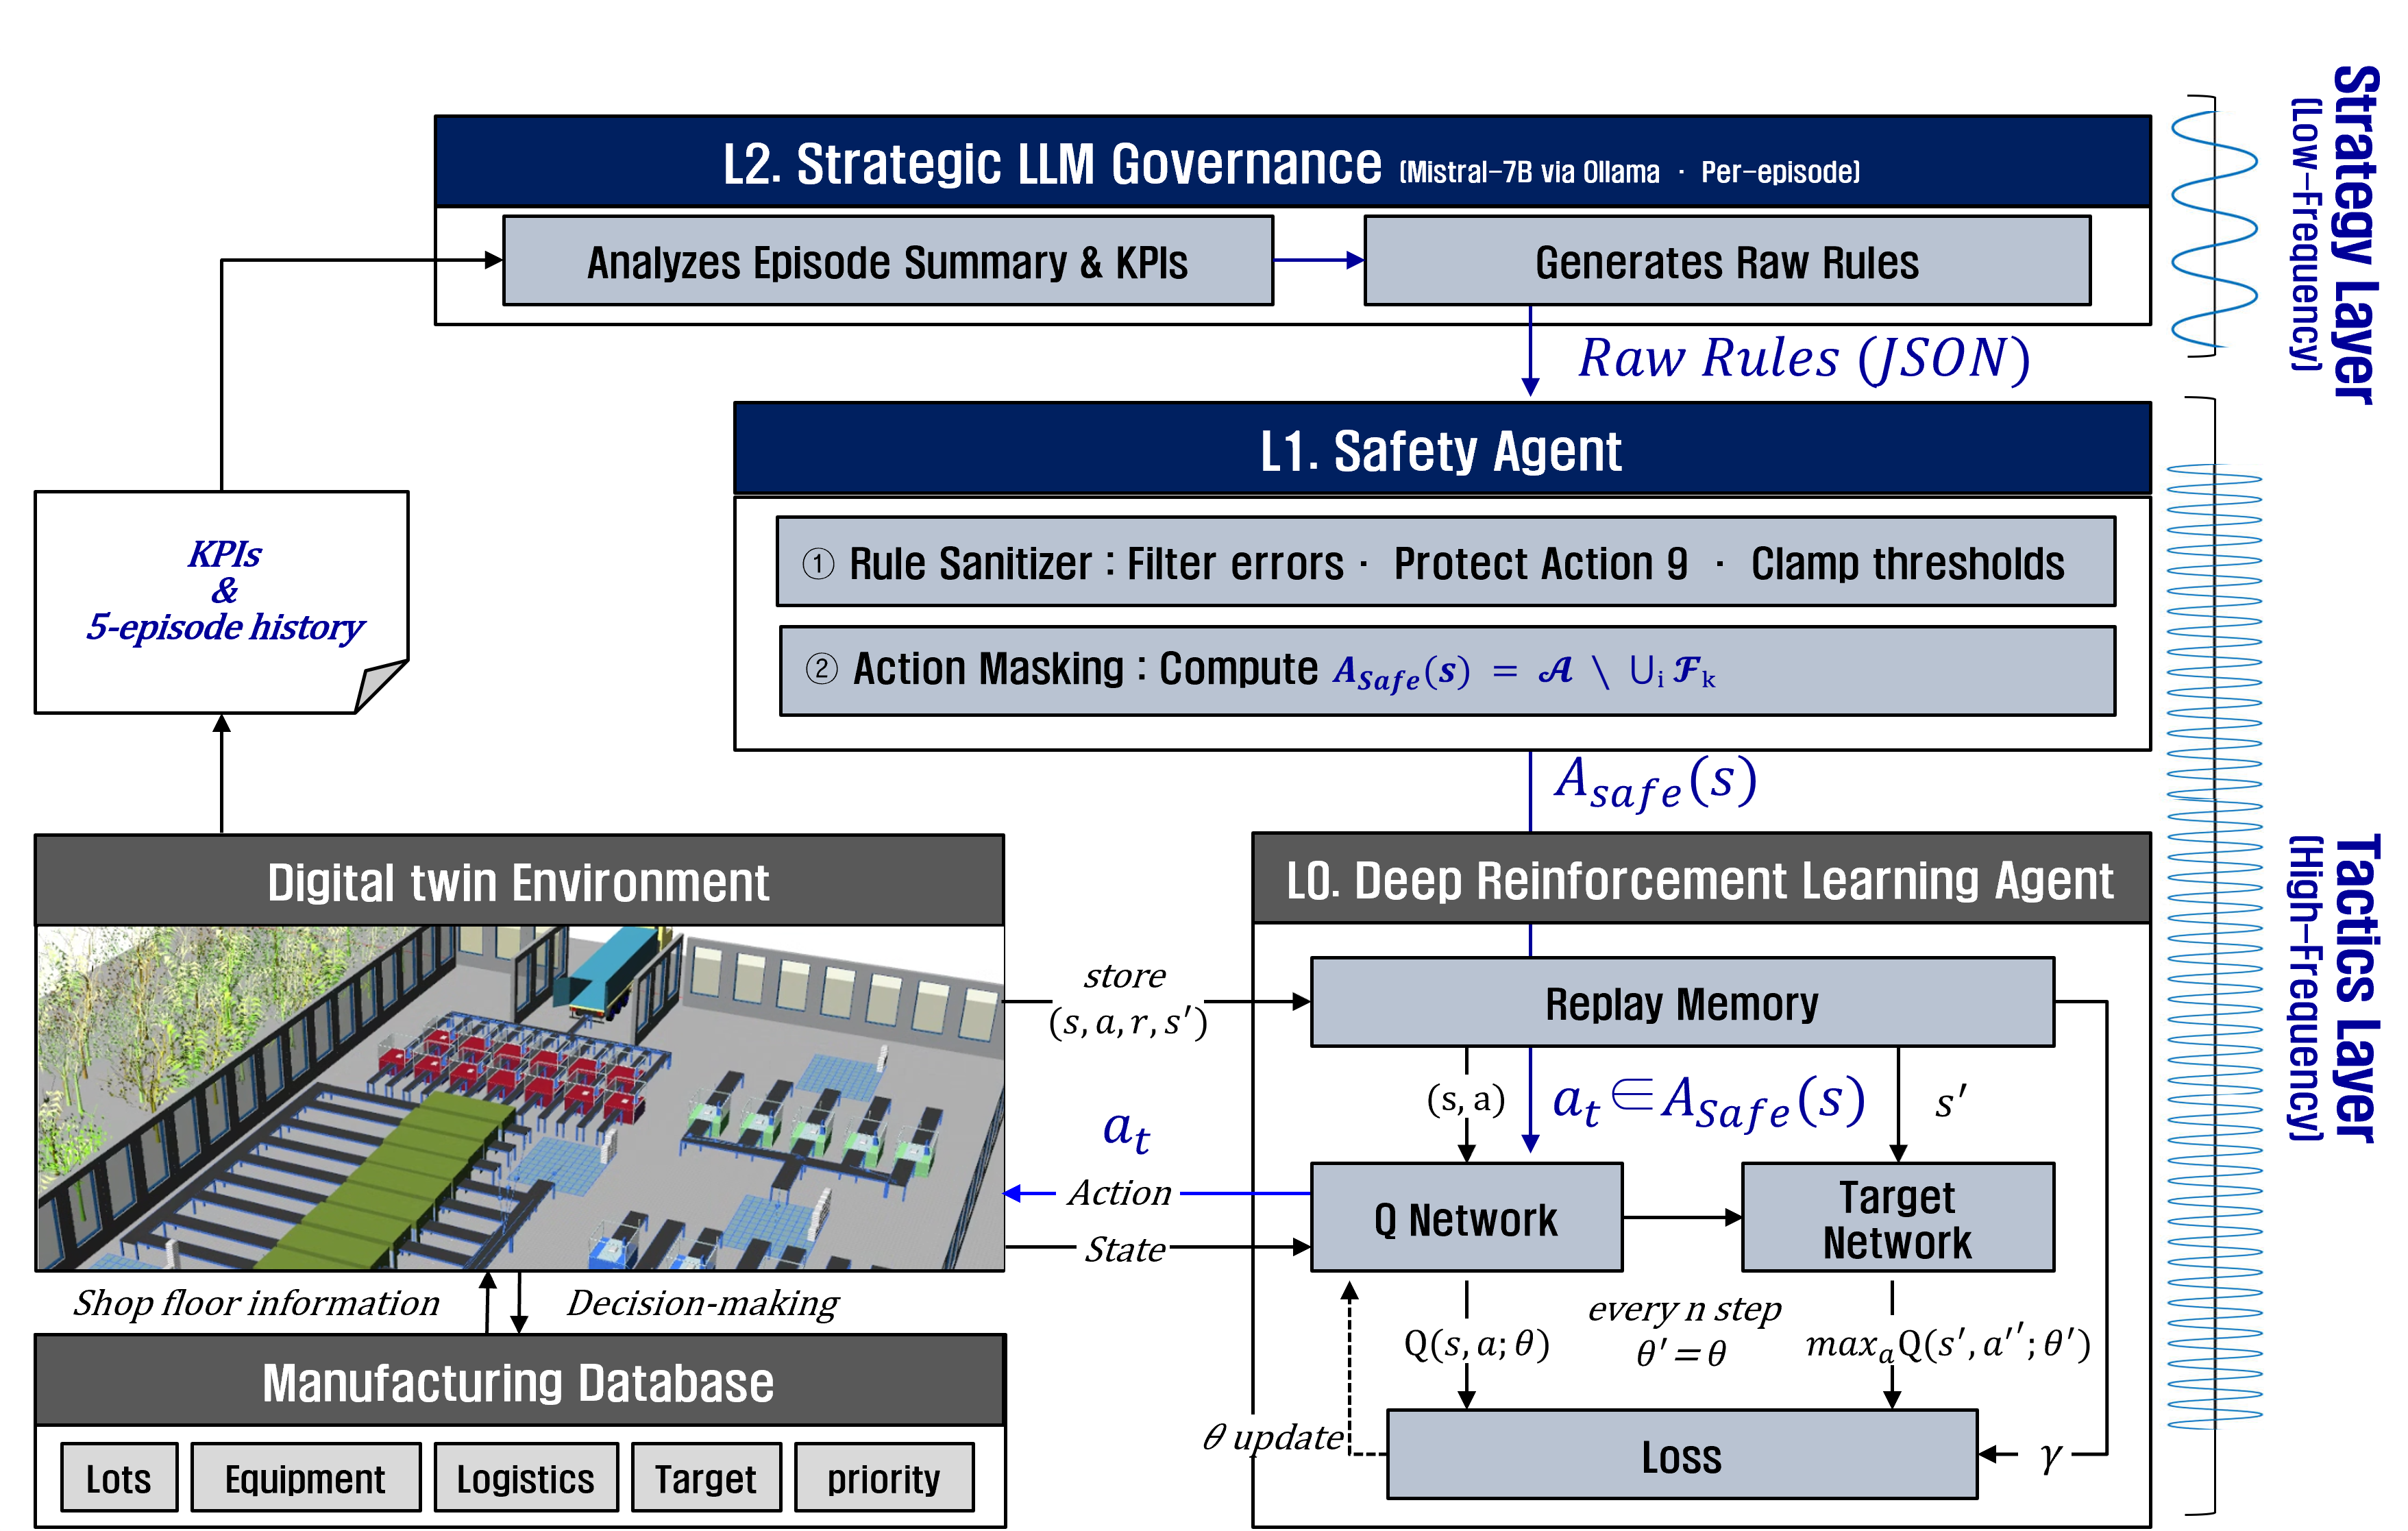
\includegraphics[width=0.98\linewidth]{fig2_architecture_improved}
    \caption{3계층 거버넌스 아키텍처. L2(Mistral-7B via Ollama)는 KPI로부터
    에피소드 단위 안전 룰을 생성하고, L1(안전 에이전트)은 내장 새니타이저를
    통해 룰을 검증하고 스텝별 행동 마스크를 집행하며(식~\ref{eq:mask}),
    L0(Rainbow DQN)는 허용된 행동 중 최고 가치 행동을 선택한다
    (식~\ref{eq:constrained}). 하드 제약 하한선은 거버넌스가 생산 달성률을
    희생하지 않도록 보장한다.}
    \label{fig:arch}
\end{figure}

Figure~\ref{fig:arch}는 서로 다른 시간 척도에서 운영되는 세 계층에 걸쳐
\emph{전략}과 \emph{전술}을 분리하는 프레임워크를 요약한다. 룰 새니타이저는
별도의 아키텍처 계층이 아닌 L1 내에 전처리 단계로 내장되어 있어, 아키텍처를
진정한 3계층으로 유지하고 추가적인 계층 간 통신 오버헤드를 방지한다.

\subsection{L2 -- 전략적 거버넌스 (로컬 LLM)}
최상위 계층은 거버넌스 체인의 진입점으로서 에피소드 단위 거버넌스를 수행하는
로컬 호스팅 LLM이다. 각 학습 에피소드 후 에피소드의 집계된 KPI---긴급 로트 수,
생산 부족 비율---와 5에피소드 롤링 히스토리를 받아,
(i) 성능 추세 분석, (ii) 지배적 병목 진단, (iii) 각각 (지표, 비교 연산자,
임계값, 금지 행동) 튜플로 지정된 안전 룰 생성을 수행한다. LLM은 자연어로
추론하고 구조화된(JSON) 응답을 반환하여, 생성하는 모든 룰에 대한 명시적이고
인간이 읽을 수 있는 근거를 제공한다.

각 에피소드는 공장 운영 하루(86,400초)를 시뮬레이션하며, 이 동안 이벤트 기반
디스패치 결정이 수백 번 발생한다. LLM 추론이 수 초 걸리는 반면 각 디스패치
결정은 밀리초 단위로 발생하므로, LLM을 스텝별 제어 루프에 배치하면 견딜 수 없는
지연 병목이 생긴다. 본 연구의 \emph{주파수 분리} 설계는 이를 해결한다: LLM은
\emph{에피소드당 한 번}(시뮬레이션 하루당 1번의 추론 호출) 작동하고, 결과 룰은
경량 L1 에이전트에 의해 해당 에피소드의 모든 디스패치 스텝에서 집행된다.
전략적 추론과 전술적 실행의 이 분리가 계층적 설계의 핵심 특징이다.

\subsection{L1 -- 안전 집행 (내장 새니타이저 포함)}
중간 계층은 L2로부터 룰 집합 $\mathcal{R} = \{r_1, \ldots, r_K\}$를 받아 매
디스패치 스텝에서 집행하는 경량 안전 에이전트이다. 집행 전에 \emph{내장 룰
새니타이저}가 각 입력 룰을 검증하여, 논리적으로 역전된 조건자를 폐기하고,
긴급 랏 우선순위 행동의 억제를 방지하며, 임계값을 스텝별 평가 척도로 클램핑한다.

각 검증된 룰 $r_k$는 튜플 $(m_k,\, \odot_k,\, \theta_k,\, \mathcal{F}_k)$이며,
$m_k$는 KPI 지표, $\odot_k \in \{>, \geq, <, \leq\}$는 비교 연산자, $\theta_k$는
임계값, $\mathcal{F}_k \subseteq \mathcal{A}$는 룰이 발동될 때 금지된 행동 집합이다.
각 디스패치 스텝에서 \emph{안전 행동 집합}은 다음과 같다:
\begin{equation}
  A_{\text{safe}}(s) \;=\; \mathcal{A} \;\setminus\;
  \bigcup_{k:\; m_k(s)\,\odot_k\,\theta_k} \mathcal{F}_k,
  \label{eq:mask}
\end{equation}
그리고 L0는 다음을 선택한다:
\begin{equation}
  a^* \;=\; \arg\max_{a \,\in\, A_{\text{safe}}(s)} Q(s, a;\,\theta).
  \label{eq:constrained}
\end{equation}
$A_{\text{safe}}(s) = \emptyset$인 경우(충돌하는 룰이 모든 행동을 금지),
폴백이 제약 없는 탐욕적 행동으로 되돌아가 데드락을 방지한다.
안전 에이전트는 무시할 수 있는 지연을 추가하며 완전히 결정론적이고 감사 가능하다.

\subsection{L0 -- 전술 에이전트 (Rainbow DQN)}
최하위 계층은 L1이 정의한 안전 행동 집합 내에서 작동하는 Rainbow DQN
에이전트\cite{hessel2018}이다. 21차원 상태 벡터 $s \in \mathcal{S}$를 관찰하고
매 결정 스텝에서 10개의 디스패칭 행동 중 하나를 선택한다.
상태는 다음을 연결한다: 정규화된 시뮬레이션 시간(1), 디바이스 패밀리별 공정 단계
버퍼 점유율(4), 디바이스별 생산 부족(4), 공정 내 리드타임 위험 통계(8),
임계 공정 단계에서 대기 중인 긴급 로트 수(4). 10개의 행동은 두 가지 범주로 구성된다.
첫 번째 범주는 \textbf{9개의 생산 디스패칭 행동}으로, 세 가지 로트 정렬 기준(생산 수량 부족 기준, 경과 대기 시간 기준, 잔여 마감 근접도 기준)과 세 가지 설비 할당 파라미터의 조합으로 구성되며, 처리량 및 TMR 최적화를 위한 9가지 정책을 제공한다.
두 번째 범주는 단일 \textbf{긴급 랏 우선순위 행동}으로, 모든 긴급 로트에 최고 디스패치 우선순위를 부여하여 일반 대기열 순서를 완전히 재정의하는 유일한 메커니즘이다.
이 설계는 의도적인 트레이드오프를 반영한다: 에이전트는 매 디스패치 스텝에서 현재 공장 상태에 따라 생산 처리량 최적화와 긴급 랏 수요 처리 중 어느 것을 우선할지 선택해야 한다. 보상 함수는 다음과 같이 분해된다:
\begin{equation}
  R(s,a) \;=\; R_{\text{prod}}(s,a) \;+\; R_{\text{urgent}}(s,a) \;+\; R_{\text{penalty}}(s,a),
  \label{eq:reward}
\end{equation}
여기서 $R_{\text{prod}}$는 생산 달성률, $R_{\text{urgent}}$는 긴급 로트 사이클
타임 감소에 대한 보상, $R_{\text{penalty}}$는 우선순위 위반에 대한 스텝별 페널티를
포착한다. 긴급 로트가 전체 로트의 최대 7.7\%에 불과하므로 $R_{\text{urgent}}$는
간헐적이고 총 반환의 작은 부분만 기여하여, Section~\ref{sec:results}에서 연구하는
희소 신호 조건을 만든다.

\subsection{하드 제약 및 생산 하한선}
L1 내의 \emph{하드 제약}은 생산 달성률이 85\% 하한선 아래로 떨어질 때마다
모든 활성 룰을 지워, 거버넌스가 긴급 로트 성능 추구 과정에서 주요 생산 목표를
희생하지 않도록 보장한다.
내장 검열기(Section~\ref{sec:lessons})와 함께 이 가드레일은 불완전한 언어 모델을
제어 루프에 안전하게 배포하는 ``결함 제거'' 수단이다.

% ============================ 4. 실험 환경 및 설정 ============================
\section{실험 환경 및 설정}
\label{sec:setup}

\subsection{디지털 트윈 및 로컬 LLM}
6개의 순차적 공정(A--F)과 임계 단계에서의 이종 장비를 갖춘 반도체 라인의
Siemens Tecnomatix Plant Simulation 모델을 사용한다.
본 모델은 실제 반도체 공장 데이터---실측 로트 도착 분포, 장비 처리 시간,
라우팅 제약---를 기반으로 구축되었으며, 소스 공장의 실제 처리량 및 사이클
타임 통계와 비교 검증되었다.
Siemens Tecnomatix Plant Simulation은 반도체 및 전자 제조 분야에서 널리 채택된
ISO\,9001 인증 상용 이산 이벤트 시뮬레이션 플랫폼으로~\cite{siemens2023tecnomatix},
라이브 공장 직접 실험의 안전·접근 위험 없이 공장 현장 동태의 신뢰 가능한
고충실도 프록시를 제공한다.
모델은 로트 도착, 라우팅, 가공, 버퍼링을 1일 시뮬레이션 지평선에 걸쳐 재현한다.

연구 환경 보안 정책으로 인해 외부 서비스로 생산 데이터를 전송하는 상용 LLM API를
사용할 수 없다; 이 제약은 실제 반도체 팹의 일반적인 데이터 거버넌스 요건도
반영한다. 따라서 Ollama 런타임을 통해 Mistral-7B~\cite{jiang2023}를 L2 거버너로 로컬 배포한다.
구조화된 JSON 룰 생성에 충분한 지시 추종 능력과 소비자 GPU 메모리 적합성을 갖추면서
에피소드당 추론 지연을 5초 이내로 유지하는 능력을 기준으로 선택되었다.
거버넌스 프레임워크는 모델에 구애받지 않으며, 더 큰 지시 튜닝 모델로의 업그레이드는
아키텍처 변경 없이 관찰된 14.5\% 룰 오류율을 낮출 것으로 기대된다.

\subsection{긴급 로트 시나리오}
\label{sec:urgentscenario}
소수의 긴급 로트(``U''로 시작하는 식별자)가 라인 입구에 주입되어 가능한 한
빠르게 완료에 도달해야 한다.
반도체 현장에서 긴급 로트는 평가 로트, 고객 샘플, 크리티컬 아이템, 긴급 계획
발주 등 다양한 운영 원천에서 발생한다. 정확한 비율은 현장마다 다르고 상업적으로
민감하므로, 본 연구에서는 산업 현장 관행에 부합하는 대표값으로 전체 로트의
$\approx$7.7\%(258개 중 20개)를 설정하였다.
이 밀도에서 긴급 로트는 병목 단계에서 빈번한 스케줄링 충돌을 유발하며,
보상 신호 대비 긴급 처리 신호가 희소해져 DRL 단독으로는 치명적 실패가
시작된다. 이 조건이 신뢰성 연구의 \emph{주요 시나리오}이다.

시뮬레이터는 긴급 랏 우선순위 행동이 일반 대기열 순서보다 긴급 로트를 앞으로 이동시킬 수 있는
\emph{유일한} 메커니즘이 되도록 구성된다. 이 설계 선택은 실험 유효성에 결정적이다:
LLM-HRL 하에서 관찰되는 긴급 로트 사이클 타임 감소가 별도의 자동 우선순위 경로가
아닌, 거버넌스 계층의 DRL 정책에 대한 영향에 기인함을 보장한다.

\subsection{지표 및 실패 정의}
\textbf{주요 지표}는 \emph{긴급 로트 사이클 타임}(CT)이다. 결과가 분포적이므로,
\emph{치명적 실패 지표}를 다음과 같이 정의한다:
\begin{equation}
  F_i \;=\; \mathbf{1}\bigl[\,\overline{\mathrm{CT}}_i > \tau\,\bigr], \qquad \tau = 3{,}500\,\text{s},
  \label{eq:failure}
\end{equation}
여기서 $\overline{\mathrm{CT}}_i$는 실행 $i$의 평균 평가 CT이다.
임계값 $\tau=3{,}500$\,s는 시뮬레이션 구성에서 파생된 \emph{사전적(a priori)} 설정값이다.
이 값의 적절성은 사후적으로도 확인된다: 경험적 CT 분포가 이 지점에서 자연적인
간격을 사이에 두고 두 개의 명확히 분리된 군집을 형성하며
(Figure~\ref{fig:ctdist}), $\tau \in [3{,}500,\,4{,}000]$\,s 범위 전반에서
Pure DRL 60\% 대 LLM-HRL 0\%라는 결론은 변하지 않는다.
$N$개의 독립 실행에 걸친 경험적 실패율은 $\hat{\rho} = \frac{1}{N}\sum_{i=1}^N F_i$이다.

\subsection{조건}
\emph{동일한 보상 함수}를 공유하고 거버넌스에서만 다른 두 조건을 비교한다:
(i) \textbf{Pure DRL}---L1/L2 계층 없는 Rainbow DQN; (ii)
\textbf{LLM-HRL (제안)}---전체 3계층 프레임워크.

\subsection{신뢰성 프로토콜}
단일 실행 비교는 신뢰할 수 없으며\cite{henderson2018}, 분포적 불확실성 정량화가
권장된다\cite{agarwal2021}. 이 모범 사례에 따라 각 조건을 5개의 독립 시드로
실행하고 \emph{실패율}과 분산을 보고한다.
디지털 트윈이 내부적으로 비결정적이므로(Section~\ref{sec:nondeterminism}),
고정된 시드조차 재현성을 보장하지 않는다. 따라서 결과의 분포를 얻으려면
복수의 독립 시드가 필요하다.
각 실행은 총 100 에피소드를 실행한다. Figure~\ref{fig:convergence}는 두 시드의
보상 곡선이 모두 에피소드 70 이전에 안정됨을 보여주므로, 마지막 30 에피소드
(에피소드 71--100)가 수렴 후 정착된 행동을 포착한다. 평가 지표는 이 구간에서
수집되며, 이 기간 동안 LLM이 생성한 룰은 동결되고
에이전트는 탐욕적으로 행동한다.

\begin{figure}[h]
    \centering
    
\includegraphics[width=0.98\linewidth]{fig_convergence}
    \caption{두 Pure-DRL 실행(시드 42 및 123, 긴급 로트 20개, 100 에피소드).
    두 곡선 모두 에피소드 70 경계(점선) 이전에 안정되어, 100 에피소드와
    30 에피소드 평가 구간이 수렴 후 정착된 행동을 포착하기에 충분함을 확인한다.
    평가 CT의 차이---한 실행 실패($>$3{,}500\,s), 다른 실행 성공---는
    Section~\ref{sec:nondeterminism}의 비결정성 분석을 동기화한다.}
    \label{fig:convergence}
\end{figure}

\subsection{에이전트 설정}
전술 에이전트는 숨겨진 레이어 [1024, 512, 256], 학습률 $3\times10^{-4}$,
할인 $\gamma=0.98$, 재플레이 용량 100k, 다단계 $n=3$, 300스텝마다 타겟 업데이트를
사용하는 Rainbow DQN이다. 모든 하이퍼파라미터는 Rainbow DQN 기본값\parencite{hessel2018}을
따르며 모든 조건에서 고정된다.

% ============================ 5. 결과 ============================
\section{결과}
\label{sec:results}

\subsection{디지털 트윈 비결정성}
\label{sec:nondeterminism}
\begin{figure}[thb]
    \centering
    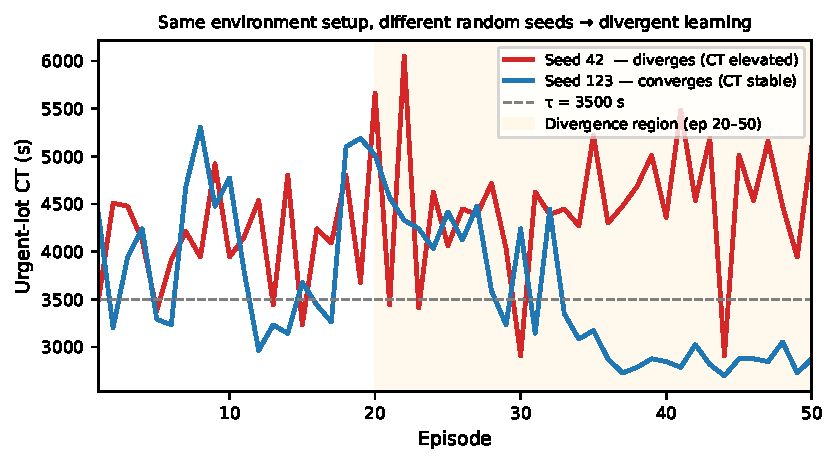
\includegraphics[width=0.98\linewidth]{fig_nondeterminism}
    \caption{\emph{동일한} 랜덤 시드와 설정(긴급 로트 20개, 50 에피소드)에서의
    두 Pure-DRL 실행. 두 실행 모두 거의 동일한 CT 궤적에서 출발하지만,
    Python RNG 외부에 존재하는 시뮬레이터 수준의 확률적 타이밍 차이가
    학습을 통해 증폭되어 에피소드 20--25 구간에서 발산한다.
    실행~A는 통과 정책으로 수렴(평가 CT~2{,}274\,s)하고, 실행~B는
    실패 정책에 정착(평가 CT~3{,}706\,s $> \tau$)한다.
    동일한 시드로도 정반대의 결과가 나올 수 있음을 보임으로써,
    비결정성이 시딩의 산물이 아닌 디지털 트윈에 내재적임을 확립한다.}
    \label{fig:nondeterm}
\end{figure}

디지털 트윈의 비결정성이 시뮬레이터 내부에서 기인함을 확립한다.
Python 수준 난수 생성기를 \emph{동일하게} 시드한 두 실행이 처음
약 20 에피소드 동안 거의 동일한 궤적을 공유하다가 발산한다
(Figure~\ref{fig:nondeterm}): Python RNG에는 보이지 않는 시뮬레이터 수준의
미세한 타이밍 차이가 학습 과정을 통해 증폭되어, 통과 사이클 타임(2{,}274\,s)으로
수렴하는 실행과 실패 임계값 위에 머무는 실행(3{,}706\,s)으로 갈라진다.
거버넌스 계층이 감내해야 할 결함은 따라서 구현 방식의 산물이 아니라
디지털 트윈의 확률적 동역학에 내재한다.

\subsection{신뢰성: 실패율 및 분산}
\begin{table}[thb]
\centering
\setlength{\tabcolsep}{4pt}
\caption{주요 시나리오의 신뢰성 결과 (긴급 로트 20개, $N=5$ 시드).}
\label{tab:reliability}
\begin{tabular}{@{}l@{\hspace{4pt}}c@{\hspace{4pt}}c@{\hspace{4pt}}c@{\hspace{4pt}}c@{}}
\toprule
\textbf{조건} & \textbf{실패율} & \textbf{CT 평균} & \textbf{CT 표준편차} & \textbf{최악} \\
\midrule
Pure DRL        & 60\% & 3{,}819\,s & 914\,s & 4{,}554\,s \\
LLM-HRL (제안)  & \textbf{0\%} & \textbf{3{,}071\,s} & \textbf{248\,s} & \textbf{3{,}309\,s} \\
\bottomrule
\multicolumn{5}{@{}l@{}}{\footnotesize $p{=}0.010$ 이항검정; $\Delta$CT $-19.6\%$; 분산 감소 $73\%$}\\
\end{tabular}
\end{table}

\begin{figure}[thb]
    \centering
    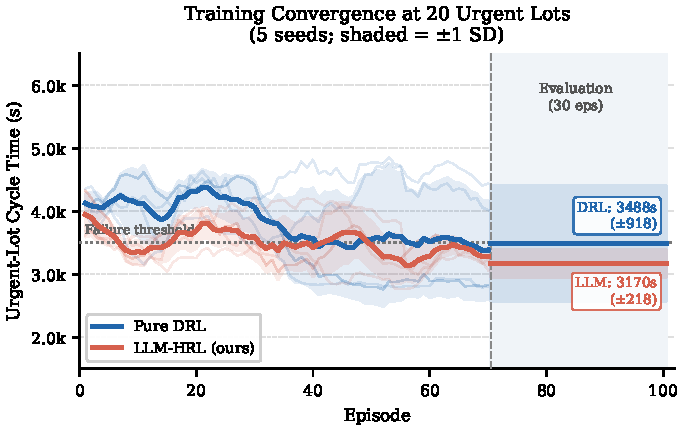
\includegraphics[width=0.98\linewidth]{fig_mechanism}
    \caption{20개 긴급 로트에서의 학습 수렴(5 시드; 음영 띠 = $\pm$1\,SD).
    두 조건 모두 에피소드 70 이전에 안정되어, 마지막 30 에피소드 평가 구간이
    수렴 후 정착된 행동을 포착함을 확인한다.
    Pure DRL 평균은 높고 가변적인 채 유지되는 반면(평가 CT 3{,}488\,s\,$\pm$918\,s),
    LLM-HRL은 모든 시드에서 실패 없이 낮고 안정적인 사이클 타임으로 꾸준히 수렴한다
    (평가 CT 3{,}170\,s\,$\pm$218\,s). LLM은 평가 스텝의 2\% 미만에 개입하며,
    이는 거버넌스의 가치가 런타임 필터링이 아닌 학습 중 정책 형성에 있음을 나타낸다.}
    \label{fig:mechanism}
\end{figure}

Table~\ref{tab:reliability}는 주요 시나리오의 중심 결과를 보고한다.
\textbf{Pure DRL은 실행의 60\%에서 치명적으로 실패했고($\hat{\rho}_{\mathrm{DRL}} = 3/5$),
LLM-HRL은 어느 것도 실패하지 않아($\hat{\rho}_{\mathrm{LLM}} = 0/5$),
$\Delta\rho = 0.60$을 달성했다.}
단측 귀무가설 $H_0: \rho_{\mathrm{LLM}} \geq 0.60$ (LLM이 Pure DRL보다 낫지 않음)
하에서 $N=5$번의 거버넌스 실행에서 $k=0$ 실패를 관찰할 확률은
\begin{equation}
  p \;=\; \Pr(X \le 0 \mid X \sim \mathrm{Bin}(5,\,0.60))
     \;=\; (1-0.60)^5 \;\approx\; 0.010,
  \label{eq:binomial}
\end{equation}
으로, 실패율 감소가 5\% 수준에서 통계적으로 유의함을 확인한다. 평균 CT는
19.6\% 개선되었고(3{,}819\,s → 3{,}071\,s), 사이클 타임 분산은 73\% 감소했다
(표준편차 914\,s → 248\,s). 생산 달성률은 조건 간 통계적으로 변화 없었다
($p>0.05$), 거버넌스가 처리량 희생 없이 실패 꼬리를 제거함을 확인한다.

시드별 상세 결과(Figure~\ref{fig:perseed})는 개선의 성격을 보여준다.
Pure DRL이 성공하는 두 시드(예: 시드 123, $\approx$2{,}820\,s)에서 거버넌스
에이전트는 이를 근접하게 따르며, 이미 수렴 중인 실행을 거버넌스가 해치지
않음을 확인한다. Pure DRL이 실패하는 세 시드(42, 2024, 7; CT $>4{,}400$\,s)에서
거버넌스 에이전트는 최선의 DRL 실행보다 높지만 실패 임계값보다 훨씬 낮은
2{,}800--3{,}300\,s 범위의 CT를 달성한다. 거버넌스는 성능 최적화기가 아니라
실패 방지기이다.

\begin{figure}[thb]
    \centering
    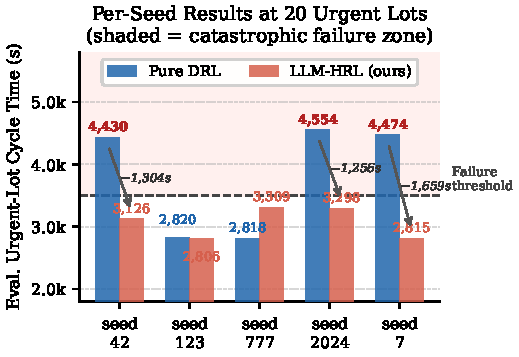
\includegraphics[width=0.98\linewidth]{fig_perseed}
    \caption{주요 시나리오(긴급 로트 20개)의 시드별 평가 CT. 빨간 음영은
    치명적 실패 영역(CT $>$ 3{,}500\,s)을 표시한다. Pure DRL은 세 시드(42, 2024, 7)에서
    실패하는 반면 LLM-HRL은 모든 5개에서 임계값 아래 유지된다.}
    \label{fig:perseed}
\end{figure}

\subsection{거버넌스 하에서의 생산 달성률}
Table~\ref{tab:tmr}은 생산 목표 달성률(TMR)이 모든 희소성 수준에서 Pure DRL과
LLM-HRL 간에 통계적으로 구별할 수 없음을 확인한다($p > 0.05$, 두 표본 $t$-검정).
거버넌스는 처리량을 희생하지 않고 신뢰성을 향상시킨다.

\begin{table}[thb]
\centering
\caption{조건별 목표 달성률(\%) ($N=5$ 시드, 평균\,$\pm$\,SD).
모든 수준에서 통계적으로 유의한 차이 없음 ($p>0.05$).}
\label{tab:tmr}
\setlength{\tabcolsep}{5pt}
\begin{tabularx}{\columnwidth}{@{}XX@{}}
\hline
\centering\textbf{Pure DRL} & \centering\arraybackslash\textbf{LLM-HRL} \\ \hline
\centering $87.2 \pm 2.5$ & \centering\arraybackslash $86.1 \pm 2.7$ \\ \hline
\end{tabularx}
\end{table}

\subsection{희소 거버넌스가 정책을 형성하는 방법}
LLM은 스텝의 단 몇 퍼센트에서만 개입하고, 평가 중 동결된 룰은 거의 발동하지
않는다---그러나 거버넌스 에이전트는 여전히 낮고 안정적인 사이클 타임을 달성한다.
이는 거버넌스의 가치가 \emph{얼마나 자주}가 아닌 \emph{언제} 개입하느냐에 있음을
나타낸다. 평가 시점의 낮은 마스킹 비율($<$2\%)은 거버넌스의 가치가 런타임
필터링보다 학습 중 정책 형성에 있음을 확인해준다---룰이 거의 발동하지 않는
평가 시점에도 LLM-HRL의 CT 분포가 더 좁다는 관찰(Figure~\ref{fig:mechanism})과
일치한다.

\subsection{어블레이션: 적응형 LLM 거버넌스의 가치}
\label{sec:ablation}

LLM의 \emph{적응형} 룰 생성이 단순한 행동 제약의 존재와 구별되는 기여를 하는지
검증하기 위해 세 번째 조건을 도입한다: \textbf{Rule-Based}---LLM-HRL과 동일한
L1 집행 메커니즘을 사용하되, 에피소드 단위 LLM 수정 없이 도메인 지식에서 도출된
고정 룰 집합을 적용하는 거버넌스 에이전트이다.
고정 룰은 \texttt{urgent\_lot\_count\,$>$\,2}일 때 긴급 우선순위 행동을 제외한
나머지 행동을 금지하며, 이는 LLM이 자율적으로 발견하는 지배적 패턴을 반영한다.
이 조건은 LLM-HRL과 동일한 DRL 에이전트(L0) 및 동일한 룰 집행 구조(L1)를
유지하되, L2 계층만 결정론적 if-else 로직으로 대체한 것이다. 따라서 DRL 에이전트
자체를 대체하는 전통적 정적 디스패칭 룰~\cite{lee2025}과는 본질적으로 다르다.
이 어블레이션은 LLM의 에피소드 단위 적응이 단순히 룰 기반 제약의 존재를 넘어서는
부가 가치를 제공하는지를 검증한다.

\begin{table}[thb]
\centering
\footnotesize
\caption{어블레이션 결과 (긴급 로트 20개, $N=5$ 시드).
Rule-Based는 LLM 적응 없이 고정 도메인 룰을 적용하며,
LLM-HRL은 에피소드 단위로 수정된 LLM 룰을 적용한다.}
\label{tab:ablation}
\setlength{\tabcolsep}{4pt}
\begin{tabularx}{\columnwidth}{@{}Xcccc@{}}
\toprule
\textbf{조건} & \textbf{실패율} & \textbf{CT 평균} & \textbf{CT std} & \textbf{최악} \\
\midrule
Pure DRL        & 60\%          & 3{,}819\,s & 914\,s  & 4{,}554\,s \\
Rule-Based      & 60\%          & 3{,}347\,s & 543\,s  & 8{,}567\,s \\
LLM-HRL (제안)  & \textbf{0\%}  & \textbf{3{,}071\,s} & \textbf{248\,s} & \textbf{3{,}309\,s} \\
\bottomrule
\end{tabularx}
\end{table}

Rule-Based는 Pure DRL과 동일한 60\% 실패율을 보이면서도 최악의 경우 결과는
훨씬 나쁘다(8{,}567\,s vs.\ 4{,}554\,s). 이는 고정 행동 제약만으로는 신뢰성을
확보할 수 없음을 확인하며, LLM의 \emph{적응적 KPI 기반} 수정이 핵심 메커니즘임을 입증한다.

% ============================ 6. 배포 교훈 ============================
\section{배포 교훈: 로컬 LLM 룰 생성}
\label{sec:lessons}

7B 로컬 모델을 제어 룰 생성기로 운영하는 것은 체계적이고 재현 가능한 오류
패턴을 드러냈다.

\subsection{룰 형식, 오류 분류 및 완화}
각 룰은 JSON 튜플 \texttt{(metric, operator, threshold,
forbidden\_actions, rationale)}이며, rationale 문자열이 순수 DRL
정책에는 없는 인간 가독형 감사 추적을 제공한다.
대표적인 정상 룰의 예시:
\begin{quote}
\footnotesize\ttfamily
\{"metric": "urgent\_lot\_count",\\
\phantom{\{}"op": "{>}", "threshold": 2,\\
\phantom{\{}"forbidden": [0, 1, \ldots, 8],\\
\phantom{\{}"rationale": "긴급 로트 우선처리"\}
\end{quote}

608개의 룰 중 14.5\%가 하나 이상의 결함을 포함했으며, 세 가지 유형으로 분류된다
(하나의 룰이 복수의 결함을 가질 수 있으므로 유형별 비율의 합은 14.5\%를 초과한다).

\noindent\textbf{(1) 척도 혼동 (9.0\%).} LLM이 \emph{에피소드 누적} KPI 값을
L1이 \emph{스텝별 스냅샷}에 대해 평가하는 임계값에 복사하는 경우.
이러한 룰은 발동할 수 없어 거버넌스를 조용히 비활성화한다.

\noindent\textbf{(2) 역전 논리 (6.7\%).} 모델이 높을수록 나쁜 지표에
``$\leq$''/``$<$'' 연산자를 사용하여 \emph{정상} 조건에서 룰이 발동하는 경우.

\noindent\textbf{(3) 중요 행동 억제 (2.6\%).} 모델이 긴급 랏 우선순위 행동
자체를 금지하는 경우.

세 가지 유형 모두 경량 구조 검사로 탐지 가능하다: 척도 혼동은 임계값을
알려진 스텝별 KPI 범위와 비교하여 포착하고, 역전 논리는 연산자 방향이
지표의 극성과 일치하는지 검증하며, 중요 행동 억제는 금지 집합에 긴급 랏
우선순위 행동이 포함된 룰을 명시적으로 거부함으로써 탐지한다.
\emph{코드 수준 새니타이저}는 룰 수신 시점에 이 검사를 결정론적으로
적용하여 모든 결함을 L1에 도달하기 전에 수정하고, 구성에 의해 안전한
룰을 산출한다. 새니타이저는 불완전한 로컬 LLM을 제어 루프에 안전하게
배포하는 구체적인 ``결함 제거'' 메커니즘이다: 언어 모델은 전략적 의도를
제공하고, 경량 코드는 그 의도가 유효하고 안전한 룰로 표현되도록 보장한다.


% ============================ 7. 논의 ============================
\section{논의}
\label{sec:discussion}

결과는 LLM-over-DRL 거버넌스의 목적에 대한 재정의를 요구한다. 거버넌스 에이전트는
\emph{운이 좋은} Pure-DRL 실행보다 뛰어나지 않다; 둘 다 유사한 사이클 타임으로
수렴한다. 그 가치는 \emph{운이 나쁜} 실행---디지털 트윈 비결정성에서 간헐적으로
발생하는 치명적 스케줄---을 제거하는 데 있다. 제조 맥락에서 잘못 스케줄된 긴급
로트 하나가 품질 시간 위반과 수율 손실로 이어질 수 있는 경우, 실패 꼬리를
제거하는 것은 평균의 한계적 개선보다 가치 있는 경우가 많다.

이 관점은 기여를 신뢰성 공학\cite{avizienis2004}과 정렬시킨다.
Laprie 결함--오류--장애 분류체계를 적용하면: \textbf{결함(fault)}은 스케줄러가
관찰하거나 제어할 수 없는 시뮬레이터 수준의 비결정성이고;
\textbf{오류(error)}는 결함이 학습 중 보상 신호를 오염시킬 때 발생하는,
긴급 로트를 과소우선시하는 학습된 정책이며;
\textbf{장애(failure)}는 $\overline{\mathrm{CT}}_i > \tau = 3{,}500$\,s,
즉 수율 및 납기 패널티를 유발하는 서비스 수준 결과이다.
거버넌스는 결함을 제거하는 것이 아니라 결함$\to$오류$\to$장애 연쇄를 차단하는
내결함성 \emph{메커니즘}으로, 고전적 내결함성 시스템의 중복성이나 우아한 성능
저하와 유사하다. 본 연구가 단일 실행 평균이 아닌 \emph{실패율}을 보고하는 이유도
여기에 있다: 개선하고자 하는 양은 결과 분포의 특성이기 때문이다.

거버넌스 오버헤드는 무시할 수 있는 수준이다: 에피소드당 LLM 호출 1번
($\approx$2--5\,s), 일반적으로 2--4개의 룰, 그리고 마이크로초 단위의 L1 평가
비용.

어블레이션 결과가 시사하는 바는 명확하다: 고정 룰은 긴급 충돌이 없는
에피소드에서도 에이전트의 탐색을 제약하여 보상 신호를 지속적으로 왜곡한다.
Pure DRL은 탐색의 자유를 유지하여 우연히 좋은 정책을 발견할 기회가 있지만,
Rule-Based는 그 경로를 차단하여 실패 케이스의 CT가 더 극단적으로 나타난다.
LLM은 KPI가 활성 충돌을 신호할 때에만 \emph{선택적으로} 개입하여 정상 운영 중
탐색을 왜곡하지 않는다. 따라서 어블레이션은 핵심 주장을 명확히 한다: 중요한 것은
제약의 \emph{존재}가 아니라 \emph{맥락적이고 적응적인} 적용이다.

\subsection{사회기술적 배포에 대한 시사점}
3계층 아키텍처는 자연스럽게 조직적 역할에 매핑된다: L0는 자동화된 디스패처,
L1은 기계 속도로 절차적 룰을 집행하며, L2는 KPI를 검토하고 에피소드당 한 번
지침을 수정하는 \emph{교대 감독자}로 작동한다. 각 룰이 명시적인 자연어 근거를 가지므로 구조화된 감사 추적이 가능하며,
이는 순수 데이터 기반 스케줄러가 제공할 수 없는 안전 중요
제조 자동화 인증에 요구되는 추적 가능성을 지원한다. 설명 가능 AI(XAI) 관점에서도,
각 룰에 부착된 자연어 근거는 ML 전문 지식 없이도 공정 엔지니어가 거버넌스 결정을
해석할 수 있게 한다: 운영자는 \emph{왜} 특정 행동이 금지되었는지 확인하고,
해당 룰이 실제 운영 우려를 반영하는지 판단하며, 다음 에피소드 전에 재정의하거나
개선할 수 있다. 이는 블랙박스 DRL 정책이 제공하지 못하는 책임 채널을 자율
스케줄링 시스템에 도입하는 핵심 기여다.

% ============================ 8. 결론 ============================
\section{결론}
실제 반도체 공장 데이터 기반으로 구축된 고충실도 디지털 트윈 환경에서,
신뢰할 수 없는 DRL 스케줄러의 의존 가능성을 실질적으로 향상시키는
3계층 로컬 호스팅 LLM 거버넌스 HRL 프레임워크를 제시했다.
주요 시나리오(긴급 로트 20개, $N=5$ 시드)에서 거버넌스는 치명적 실패율을
60\%에서 0\%로 감소시켰고($p=0.010$, 단측 이항검정), 생산 달성률의 손실 없이
사이클 타임 분산을 73\% 감소시켰다.
두 조건의 CT 분포는 선택한 실패 임계값 $\tau=3{,}500$\,s에서 자연적인 간격으로
명확하게 분리된 군집을 형성하며, 이 결과가 임계값 선택의 인공물이 아님을 확인한다.
또한 거버넌스 효과가 런타임 제약이 아닌 DRL 학습 궤적 교정에서 비롯됨을 보였다.
7B 로컬 모델의 룰 생성 오류 패턴과 배포를 안전하게 만든 프롬프트-새니타이저
파이프라인을 추가로 보고했다. LLM 거버넌스는 성능 최적화가 아닌
사회기술적 제조 시스템에서 학습 컴포넌트를 위한 \emph{내결함성 메커니즘}으로
이해하는 것이 가장 적절하며, 고충실도 디지털 트윈과 에피소드 단위 LLM 감시의
결합은 실제 반도체 팹에서 신뢰 가능한 강화학습 배포로 나아가는 실용적인
경로를 제공한다.

% ============================ 한계 ============================
\section{한계 및 향후 연구}
\label{sec:limitations}

\textbf{디지털 트윈 충실도 대 실제 배포.}
본 연구에서 사용된 디지털 트윈은 실제 반도체 공장 데이터를 기반으로 구축되고
실제 생산 통계와 검증되어 고충실도 실험 기반을 제공한다.
그러나 모든 실험은 시뮬레이션 환경에서 수행되었으며, 실제 팹으로의 배포를 위해서는
추가적인 통합 작업, 공장 장비와의 실시간 통신 인터페이스, 그리고 공식적인
안전 자격 인증(예: 거버넌스 레이어에 대한 IEC\,61508 SIL 평가)이 필요하다.
디지털 트윈이 이미 거버넌스 대상 생산 동태를 재현하고 있으므로, 소스 공장과의
협력을 통한 실제 배포를 향후 연구로 계획하고 있으며 프레임워크의 직접 이전이
가능할 것으로 예상한다.

\textbf{단일 라인 범위.}
모델은 6개의 순차적 공정 단계를 갖는 단일 라인을 나타낸다. 라인·제품·
모델 패밀리 간 일반화는 평가되지 않았으며, 다른 팹이나 제품 조합에 방법론을
적용하려면 디지털 트윈 재보정이 필요하다.

\textbf{LLM 룰 품질.}
로컬 7B 모델은 14.5\%의 룰 오류율을 보였으며, 새니타이저 파이프라인이
런타임에서 잔여 오류를 0으로 감소시켰다. 더 큰 지시 모델로의 업그레이드 또는
도메인별 스케줄링 데이터에 대한 미세 조정이 원시 오류율 감소에 기여할 것으로
예상된다.

\printbibliography

\end{document}
